% TODO
% Add footnotes
% Print this pdf

\documentclass [12pt, letterpaper, twoside] {article}
\usepackage[utf8]{inputenc}
\usepackage [left=1.0in, right=1.0in, top=1.0in, bottom=1.0in] {geometry}
% For keeping time
\usepackage {datetime}
% For pictures/graphs
\usepackage {tikz}
% The essential math library
\usepackage {amsmath}
% To make tables
\usepackage {tabu}
% To add multiple rows or columns per table column/row
\usepackage {multirow}
\usepackage {verbatim}
% To add captions to tables
\usepackage {caption}
\usepackage {float}
% For the degree symbol
\usepackage {gensymb}
% To make graphs
\usepackage {pgfplots}

\raggedbottom
\begin {document}
\begin {titlepage}
\begin {center}
Department of Biological, Chemical, and Physical Science\\
\vspace {0.1cm}
Illinois Institute of Technology\\
\vspace {0.1cm}
General Physics I: Mechanics (PHYS 123-02)\\
\vspace* {\fill}
\begingroup
\Large
\textbf {Projectile Motion}
\vspace {0.35cm}

\normalsize
Lab 2
\vspace {1.5cm}
\endgroup
\vspace* {\fill}
\end {center}

\vspace*{\fill}
\begin {flushright}
\footnotesize
Emily Pang, Coby Schencker (lab partner)\\
Date of experiment: 30 Aug 2019\\
Due date: 5 Sept 2019\\
Lab section L04\\
TA: Mithila Mangedarage\\
Updated \usdate\today~(\currenttime)
\end {flushright}
\end {titlepage}
\subsection* {UNPROCESSED DATA}
  \begin {table}[h]
   \centering
    \begin {tabular} {| l | r | r | r |}
      \hline\hline
      Angle & 0 & 15 & 45 \\
      \hline
      \multirow {3}{*}{Distance (m)} & 1.455 & 1.664 & 1.593 \\ 
      & 1.442 & 1.679 & 1.596 \\
      & 1.460 & 1.682 & 1.617 \\
      \hline
      Avg Distance (m) & 1.452 & 1.675 & 1.602 \\
      \hline
      \multirow {3}{*}{Time (s)} & 2.426 & 2.126 & 3.876 \\
      & 1.602 & 2.463 & 3.449 \\
      & 2.131 & 2.286 & 3.706 \\
      \hline
      Avg Time(s) & 2.053 & 2.292 & 3.677 \\
      \hline\hline
    \end {tabular}
    \caption {Low power firing}
  \end {table}

  \begin {table}[h]
   \centering
    \begin {tabular} {| l | r | r | r |}
      \hline\hline
      Angle & 0 & 15 & 45 \\
      \hline
      \multirow {3}{*}{Distance (m)} & 1.907 & 2.297 & 1.392 \\ 
      & 1.911 & 2.316 & 1.402 \\
      & 1.918 & 2.321 & 1.402 \\
      \hline
      Avg Distance (cm) & 1.912 & 2.311 & 1.399 \\
      \hline
      \multirow {3}{*}{Time (s)} & 2.673 & 3.057 & 3.705 \\
      & 2.218 & 3.559 & 2.311 \\
      & 1.584 & 2.706 & 1.543 \\
      \hline
      Avg Time (s) & 2.158 & 3.107 & 2.520 \\
      \hline\hline
    \end {tabular}
    \caption {High power firing}
  \end {table}
\subsection* {Question 1}
PART A \\\\
The two initial velocities can be found by taking one of the kinematic equations
\begin {equation}
  \begin {split}
    \Delta {x} & = v_{0}t + \dfrac{1}{2}at^{2} 
  \end {split}
\end {equation}
The acceleration in the x-direction is zero, so this is the resulting equation 
\begin {equation}
  \begin {split}
    v_{0} = \dfrac{\Delta{x}}{t}
  \end {split}
\end {equation}
to find the resulting x-component of the initial velocity. In order to find initial velocity in the \(y\) component, we know this fact:
\begin {equation}
  \begin {split}
    \tan(\theta) & = \dfrac{v_{y}}{v_{x}} \\
    v_{x}\tan({\theta}) & = v_{y} \\
    v_{y} & = v_{x}\tan(\theta)
  \end {split}
\end {equation}
Table 3 shows the resulting average initial velocities for Part A of Question 1.
\begin {table}[h]
  \centering
  \begin {tabular} {| l | r | r | r |}
    \hline\hline
    Angle & 0 & 15 & 45 \\
    \hline
    Avg Initial Velocity (\(\tfrac{\text{m}}{\text{s}}\)) & 0.7283 & 0.7593 & 0.6176 \\
    \hline
    Avg \(x\) velocity (\(\tfrac{\text{m}}{\text{s}}\)) & 0.7283 & 0.7334 & 0.4367 \\
    \hline
    Avg \(y\) velocity (\(\tfrac{\text{m}}{\text{s}}\)) & 0 & 0.1965 & 0.4367 \\
    \hline
    Time (s) & 2.053 & 2.292 & 3.677 \\
    \hline
    Horizontal Distance (m) & 1.452 & 1.675 & 1.602 \\
    \hline\hline
  \end {tabular}
  \caption {Initial velocities for the low power firing}
\end {table}

\begin {table}[h]
  \centering
  \begin {tabular} {| l | r | r | r |}
    \hline\hline
    Angle & 0 & 15 & 45 \\
    \hline
    Avg Initial Velocity (\(\tfrac{\text{m}}{\text{s}}\)) & 0.9286 & 0.7799 & 0.8914 \\
    \hline
    Avg \(x\) velocity (\(\tfrac{\text{m}}{\text{s}}\)) & 0.9286 & 0.7533 & 0.6303 \\
    \hline
    Avg \(y\) velocity (\(\tfrac{\text{m}}{\text{s}}\)) & 0 & 0.2018 & 0.6303 \\
    \hline
    Time (s) & 2.158 & 3.107 & 2.520 \\
    \hline
    Horizontal Distance (m) & 1.912 & 2.311 & 1.399 \\
    \hline\hline
  \end {tabular}
  \caption {Initial velocities for the high power firing}
\end {table}

\noindent
PART B \\\\
The angle that gave us the longest range was 15\(\degree\). To find \(y_{max}\), we use the following kinematic equation:
\begin {equation}
  \begin {split}
    v_{f}^2 & = v_{0}^2 + 2a\Delta{y} \\
    \Delta{y} & = -\dfrac{v_{0}^2}{2a} \\
  \end {split}
\end {equation}
Since the final velocity in the \(y\) direction is zero, we can cancel it out. Thus, the \(y_{max}\) for the low power firing is
\begin {equation}
  \begin {split}
    \Delta{y} & = \dfrac{(0.1965\tfrac{\text{m}}{\text{s}})^2}{2(9.8\tfrac{\text{m}}{\text{s}^2})}\\ 
    \Delta{y} & = 0.0020\text{ m} \\
  \end {split}
\end {equation}

\noindent
and we do the same for the high power firing here.
\begin {equation}
  \begin {split}
    \Delta{y} & = \dfrac{(0.2018\tfrac{\text{m}}{\text{s}})^2}{2(9.8\tfrac{\text{m}}{\text{s}^2})}\\ 
    \Delta{y} & = 0.0021\text{ m} \\
  \end {split}
\end {equation}
The final \(y_{max}\) is then 0.0021 plus the initial height, 1.1 m. We also know that to find the angle with the highest \(y_{max}\), we have to find out what \(y_{max}\) is with \(\theta\) equaling 45\(\degree\). We first find out what \(y_{max}\) is for the lower power firing, which ends up as
\begin {equation}
   \begin {split}
     \Delta{y} & = \dfrac{(0.4367\tfrac{\text{m}}{\text{s}})^2}{2(9.8\tfrac{\text{m}}{\text{s}^2})}\\
     \Delta{y} & = 0.009730 \text{ m} \\
   \end {split}
 \end {equation}
And for the high power firing:
\begin {equation}
   \begin {split}
     \Delta{y} & = \dfrac{(0.6303\tfrac{\text{m}}{\text{s}})^2}{2(9.8\tfrac{\text{m}}{\text{s}^2})}\\
     \Delta{y} & = 0.02027 \text{ m} \\
   \end {split}
 \end {equation}
 As evidenced by the results for the two calculations, \(y_{max}\) is the highest when \(\theta\) = 45\degree. \\\\

\noindent
PART C

\begin {center}
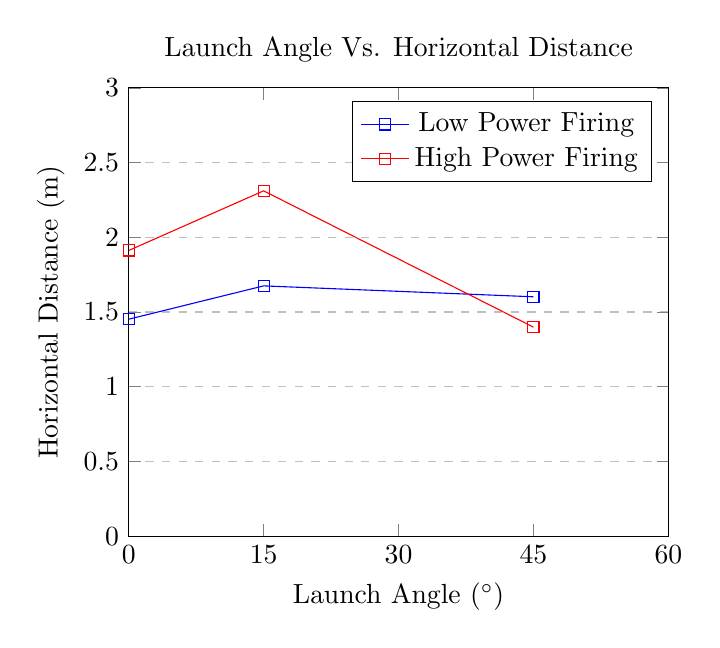
\begin{tikzpicture}
\begin{axis}[
    title={Launch Angle Vs. Horizontal Distance}, 
    xlabel={Launch Angle (\(\degree\))}, 
    ylabel={Horizontal Distance (m)}, 
    xmin=0, xmax=60,
    ymin=0, ymax=3,
    xtick={0,15,30,45,60},
    ytick={0,0.50,1,1.50,2,2.50,3},
    legend pos=north east,
    ymajorgrids=true,
    grid style=dashed,
]
 
\addplot[color=blue, mark=square,]
  coordinates {(0,1.452)(15,1.675)(45,1.602)};

\addplot[
  color=red,
  mark=square,]
  coordinates {(0,1.912)(15,2.311)(45,1.399)};
  \legend{Low Power Firing,High Power Firing}

\end{axis}
\end{tikzpicture}
\end {center}

\noindent
PART D \\\\

\noindent
To calculate the acceleration due to gravity, we can use the experiments where the angle \(\theta\) was equal to 0\degree. For this, we can use the following kinematic equation:
\begin {equation}
  \begin {split}
    \Delta{y} & = v_{0}t-\dfrac{1}{2}at^2 \\
    a & = \dfrac{-2\Delta{y}}{t^2} \\
  \end {split}
\end {equation}
With this equation, we get -1.043 \(\tfrac{\text{m}}{\text{s}^2}\) and -0.4724 \(\tfrac{\text{m}}{\text{s}^2}\). No, this is not at all close to the accepted value of 9.8 \(\tfrac{\text{m}}{\text{s}^2}\). Possible errors include the fact that we had to measure the height of the ball launcher after the fact and the timer didn't seem to work for the entirety of our experiments. In fact, these are definite errors. \\\\ 

\noindent
PART E \\\\
To find the time it would take for the ball to reach the ground, we first have to find the \(y_{max}\) and calculate the times separately. The first kinematic equation involved is this one, where the final velocity is zero:
\begin {equation}
  \begin {split}
    v_{f} & = v_{0} + at \\
    t & = \dfrac{-v_{0}}{a} \\
  \end {split}
\end {equation}
The average initial velocity for the low power firing is about 0.7017 \(\tfrac{\text{m}}{\text{s}^2}\) and 0.8665 \(\tfrac{\text{m}}{\text{s}^2}\) for the initial high power firing velocity. So the times going up would be 0.07160 and 0.08842 seconds respectively. For the times going downwards, we first have the find the change in \(y\) distance. We then combine the equations to make it easier than solving one after the other.
\begin {equation}
  \begin {split}
    v_{f}^2 & = v_{0}^2 + 2a\Delta{y} \\
    \Delta{y} & = \dfrac{-v_{0}^2}{2a} \\
  \end {split}
\end {equation}
The equation for the time going down:
\begin {equation}
  \begin {split}
    \Delta{x} & = v_{0}t+\dfrac{1}{2}at^2 \\
    \dfrac{-v_{0}^2}{2a}+1.1\text{m} & = \dfrac{1}{2}at^2 \\
    t & = \sqrt{\dfrac{2(\tfrac{v_{0}^2}{2a}+1.1\text{m})}{a}} \\
    t & = \sqrt{\dfrac{\tfrac{v_{0}^2}{a}+2.2\text{m}}{a}} \\
  \end {split}
\end {equation}
For the times going downwards, we calculate 0.4792 seconds and 0.4820 for the two firing speeds respectively. Together, the time it takes for the low power firing is 0.5508 and 0.5704 seconds for the high power firing.

\subsection*{Question 2}
Ideally, the mathematical curve of the projectile motion trajectory is parabolic. For instance, two examples of this parabolic shape that I have seen are when I play badminton and I am serving the shuttlecock. Although the shuttlecock is aerodynamically different than a ball, it doesn't quite have a parabolic path. \\
Another example is when I see someone accidentally hit their phone while on a bridge, giving it an initial velocity. The phone's fall is similar to a parabolic line, falling to its death when it reaches the ground. However, for both of these and especially for the badminton example, the objects are affected by air resistance, and the line of their motion will likely not be perfectly parabolic. \\

\subsection* {Question 3}
Yes, there are two different angles that would give the same range. These are complimentary angles, or angles that add up to 90\degree. This makes sense, because the \(x\) and \(y\) components of velocity are the same when \(\theta\) is 45\degree, and so must meet each other along all other angles. However, there are no two angles that give the same height, because as \(\theta\) increases, so does the height.

\subsection* {Question 4}
If the ball were launched horizontally from the launcher, it's time would be equal to taking the entire initial velocity and using kinematics equations. We actually did this in our experiment, and it took 2.053 seconds on average for the low power and 2.158 seconds on the high power. However, if we simply dropped the ball from the height of the launcher, we would get the same times due to the fact that the starting heights are the same, the accelerations are the same, and the \(x\) direction does not affect the \(y\) direction.

\end {document}
